\documentclass{beamer}

\mode<presentation>
{
  \usetheme{Frankfurt}
  \usecolortheme{orchid}
  \setbeamercovered{invisible}
  \setbeamertemplate{footline}[frame number]
}

\usepackage[english]{babel}
\usepackage[latin1]{inputenc}
\usepackage{times}
\usepackage[T1]{fontenc}
\usepackage{tikz}
\usepackage{array}
\usepackage{cancel}


\usetikzlibrary{shapes,backgrounds}

\def\multiset#1#2{\ensuremath{\left(\kern-.3em\left(\genfrac{}{}{0pt}{}{#1}{#2}\right)\kern-.3em\right)}}

\def\blue{\color{blue}~}
\def\black{\color{black}~}
\def\bl[#1]#2{\begin{block}{#1}#2\end{block}}
\def\integers{\mathbb{Z}}
\def\enumb{\begin{enumerate}}
\def\enume{\end{enumerate}}
\def\itemb{\begin{itemize}}
\def\iteme{\end{itemize}}
\def\div{~\textrm{div}~}
\def\mod{~\textrm{mod}~}


\usepackage{remreset}
\makeatletter
\@removefromreset{subsection}{section}
\makeatother
\setcounter{subsection}{1}

\title{Discrete Mathematics, Section 001, Fall 2016}
\subtitle{Lecture 23: Connections, Trees}

\author[Zsolt]{Zsolt Pajor-Gyulai \\ \texttt{zsolt@cims.nyu.edu}}

\pgfdeclareimage[height=1cm]{NYUlogo}{NYUlogo.jpg}

\institute[NYU] 
{
\normalsize Courant Institute of Mathematical Sciences
}
\titlegraphic{\pgfuseimage{NYUlogo}}

\begin{document}

\begin{frame}
  \titlepage
\end{frame}

\AtBeginSection[]
{
\begin{frame}
\frametitle{Outline}
\tableofcontents[currentsection]
\end{frame}}

\section{Walks, Paths}

\begin{frame}
\bl[Definition]{Let $G=(V,E)$ be a graphs. A \textbf{walk} in $G$ is a sequence (or lists) if vertices, with each vertex adjacent to the next; that is,
\[
W=(v_0,v_1,\dots,v_l)\qquad v_0\sim v_1\sim v_2\sim\dots\sim v_l
\]
The \textbf{length} of this walk is $l$. }
Note that there are $l+1$ vertices on the walk.
\begin{columns}
\column{0.35\textwidth}
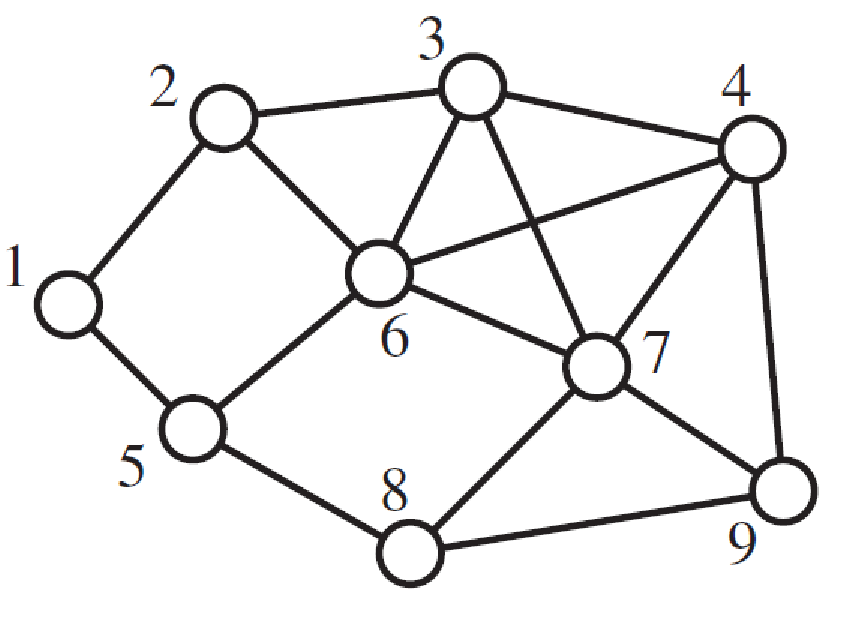
\includegraphics[scale=0.3]{WalkGraph.pdf}
\column{0.65\textwidth}
\itemb
\item $1\sim 2\sim 3\sim 4$. \vspace{-0.1cm}
\bl[]{\vspace{-0.1cm}
\[
\textrm{This is a $(1,4)$ walk.}
\]}
\item $W=1\sim 2\sim 3\sim 6\sim 2\sim 1\sim 5$.
\item $W^{-1}=5\sim 1\sim 2\sim 6\sim 3\sim 2\sim 1$.
\iteme
\end{columns}\vspace{-0.2cm}
\bl[]{If $W=v_0\sim v_1\sim\dots\sim v_{l-1}\sim v_l$, then its \textbf{reversal} $W^{-1}=v_l\sim v_{l-1}\sim\dots\sim v_1\sim v_0$ is also a walk.}
\end{frame}

\begin{frame}
\bl[Definition]{Let $G=(V,E)$ be a graphs. A \textbf{walk} in $G$ is a sequence (or lists) if vertices, with each vertex adjacent to the next; that is,
\[
W=(v_0,v_1,\dots,v_l)\qquad v_0\sim v_1\sim v_2\sim\dots\sim v_l
\]
The \textbf{length} of this walk is $l$. }

\begin{columns}
\column{0.35\textwidth}
\begin{figure}
\centering
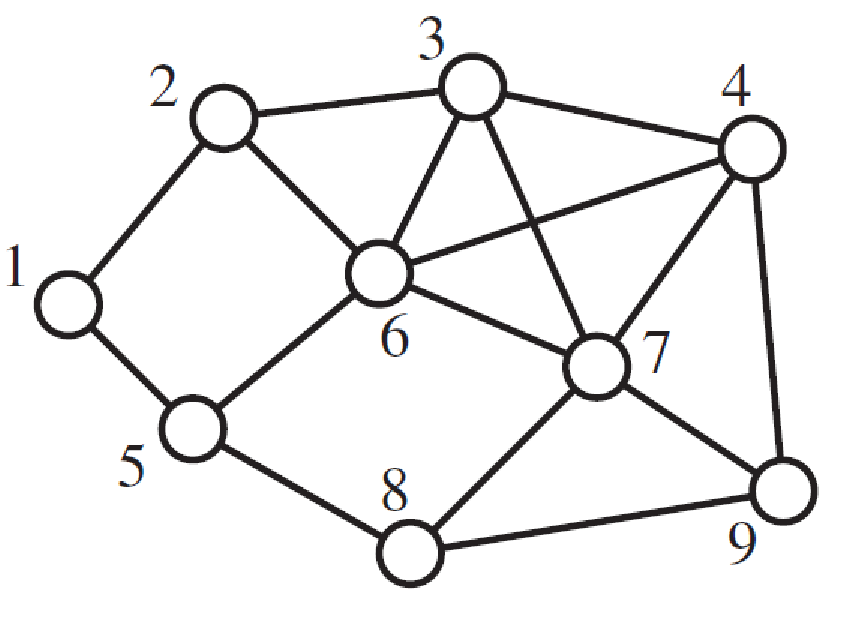
\includegraphics[scale=0.3]{WalkGraph.pdf}
\end{figure}
\column{0.65\textwidth}
\itemb
\item $9$
\bl[]{\vspace{-0.1cm}
\[
\textrm{This is a walk of length zero.}
\]}
\item $1\sim 5\sim 1\sim 5\sim 1 $
\bl[]{\vspace{-0.1cm}
\[
\textrm{This is a \textbf{closed} walk.}
\]}
\item The sequence $(1,6,7,9)$ is not a walk.
\iteme
\end{columns}
\end{frame}

\begin{frame}
\bl[Concatenation]{Let $G$ be a graph. Suppose $W_1$ and $W_2$ are the following walks:
\[
W_1=v_0\sim v_1\sim\dots\sim v_l,\qquad W_2=w_0\sim w_1\sim\dots w_k
\]
and suppose $v_l=w_0$. Their \textbf{concatenation}, denoted $W_1+W_2$, is the walk
\[
v_0\sim v_1\sim\dots\sim (v_l=w_0)\sim w_1\sim\dots\sim w_k.
\]}

\begin{columns}
\column{0.4\textwidth}
\begin{figure}
\centering
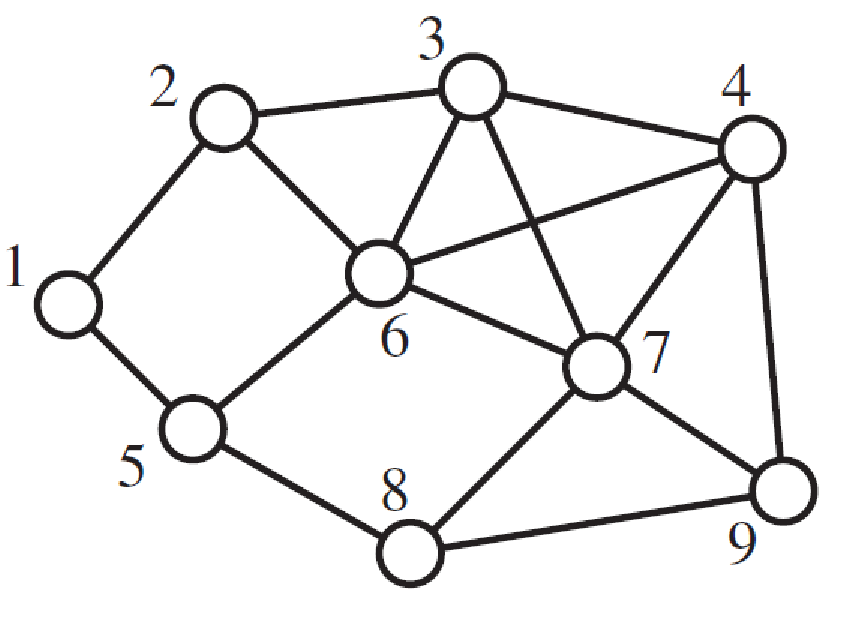
\includegraphics[scale=0.3]{WalkGraph.pdf}
\end{figure}
\column{0.6\textwidth}
The concatenation of\vspace{-0.1cm}
\[
1\sim 2\sim 3\sim 4\qquad 4\sim 7\sim 3\sim 2
\]\vspace{-0.5cm}\\
and\vspace{-0.2cm}
is
\[
1\sim 2\sim 3\sim 4\sim 7\sim 3\sim 2
\]
\end{columns}
\end{frame}

\begin{frame}
\bl[Definition]{A \textbf{path} in a graph is a walk in which no vertex is repeated.}
\begin{columns}
\column{0.4\textwidth}
\begin{figure}
\centering
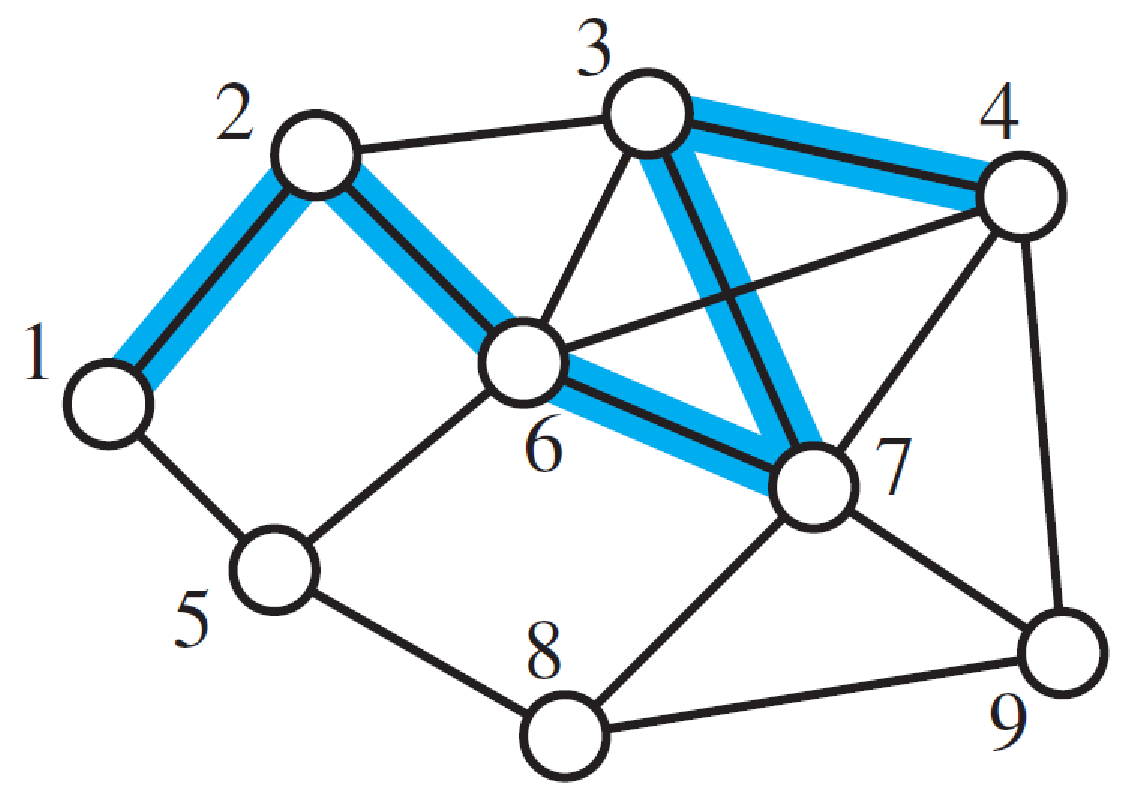
\includegraphics[scale=0.25]{PathGraph.pdf}
\end{figure}
\column{0.6\textwidth}
\itemb
\item The walk $1\sim 2\sim 6\sim 7\sim 3\sim 4$ is a path.
\item It is also called a $(1,4)$ path.
\item Note that the definition implies that no edge will be repeated either.
\iteme
\begin{center}
Do Problem 1!
\end{center}
\end{columns}
\bl[Proposition]{Let $P$ be a path in a graph $G$. Then $P$ does not traverse any edge of $G$ more than once.}
\end{frame}

\begin{frame}
\bl[Proposition]{Let $P$ be a path in a graph $G$. Then $P$ does not traverse any edge of $G$ more than once.}
Suppose FTSC that some path $P$ in a graph $G$ traverses the edge $e=uv$ more than once. Then
\begin{align*}
P&=\dots\sim u\sim v\sim\dots\sim u\sim v\sim\dots\qquad\textrm{or}\\
P&=\dots\sim u\sim v\sim\dots\sim v\sim u\sim\dots
\end{align*}
Either case, we repeated $u$ and thus $P$ is not a path. $\Rightarrow\Leftarrow$.\qed\vspace{0.3cm}\pause

We have the following alternative definition:
\bl[Definition]{ A \textbf{path} is a graph with vertex set $V=\{v_1,v_2,\dots, v_n\}$ and edge set
\[
E=\{v_iv_{i+1}: 1\leq i<n\}
\]
A path on $n$ vertices is denoted by $P_n$.}
\end{frame}

\begin{frame}{Connections}
\itemb
\item We want to capture the notion when vertices are connected.
\item Two vertices are connected if there is a path connecting them. 
\iteme
\bl[Definition]{Let $G$ be a graph and let $u,v\in V(G)$. We say that $u$ is \textbf{connected to} $v$ provided there is a $(u,v)$-path in $G$.}
\center We will show that this is an equivalence relation on $V(G)$.
\end{frame}

\begin{frame}
\bl[Theorem]{Let $G$ be a graph. The is-connected-to relation is an equivalence relation on $V(G)$.}
\itemb
\item \underline{Reflexive}:

If $v$ is a vertex, then the path $(v)$ is a $(v,v)$-path and so $v$ is connected to $v$.

\item \underline{Symmetric}:

Suppose, in a graph $G$, vertex $u$ is connected to vertex $v$. This means there is a $(u,v)$-path $P$ in $G$. Then it's reversal $P^{-1}$ is a $(v,u)$ path, and so $v$ is connected to $u$.
\item \underline{Transitive}:

Suppose $x$ is connected to $y$, which is connected to $z$. This means that there is a $(x,y)$ path $P$ and a $(y,z)$ path $Q$ in $G$. We want to show that there is also an $(x,z)$-path. The obvious candidate is the concatenation $P+Q$. 
\center This, however, doesn't work.
\iteme
\end{frame}

\begin{frame}
\bl[Theorem]{Let $G$ be a graph. The is-connected-to relation is an equivalence relation on $V(G)$.}
\itemb
\item \underline{Transitive}:

Suppose $x$ is connected to $y$, which is connected to $z$. This means that there is a $(x,y)$ path $P$ and a $(y,z)$ path $Q$ in $G$. We want to show that there is also an $(x,z)$-path. The obvious candidate is the concatenation $P+Q$. 
\begin{figure}
\centering
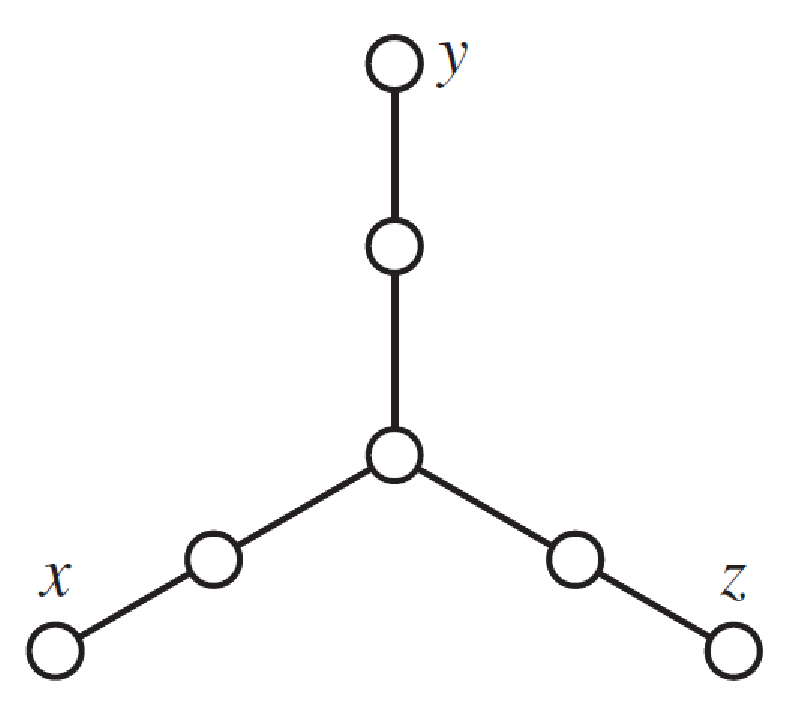
\includegraphics[scale=0.22]{PathTrans.pdf}
\end{figure}

$P+Q$ might repeat vertices and therefore it might not be a path only a walk. We need to show that we can construct a path out of it.
\iteme
\end{frame}

\begin{frame}
\bl[Lemma]{Let $G$ be a graph and let $x,y\in V(G)$. If there is an $(x,y)$-walk in $G$, then there is an $(x,y)$-path in $G$.}
~~~~Suppose there is an $(x,y)$-walk in the graph $G$. By the well ordering principle, there is a shortest $(x,y)$-walk $P$. We claim that this walk is actually a path.

~~~~Suppose FTSC, that $P$ is not an $(x,y)$-path. Then there must be a repeated vertex $u$ on the path:
\[
P=x\sim\dots ? \sim u\textcolor{blue}{\sim\dots\sim u}\sim??\sim\dots\sim y.
\]
Form a new walk $P'$ by removing the blue part. Since $u\sim ??$, $P'$ will be a walk shorter than $P$. $\Rightarrow\Leftarrow$\qed
\end{frame}

\begin{frame}
\bl[Theorem]{Let $G$ be a graph. The is-connected-to relation is an equivalence relation on $V(G)$.}
\itemb
\item \underline{Transitive}:

Suppose $x$ is connected to $y$, which is connected to $z$. This means that there is a $(x,y)$ path $P$ and a $(y,z)$ path $Q$ in $G$. We want to show that there is also an $(x,z)$-path. \textcolor{blue}{The concatenation $P+Q$ is an $(x,z)$-walk. Therefore by the Lemma, there is an $(x,z)$-path as well and thus $x$ is connected to $y$.}\qed
\iteme
\end{frame}

\begin{frame}
\bl[]{\textbf{Q}: What are the equivalence classes for this equivalence relation? }
\itemb
\item If $u$ and $v$ are in the same equivalence class then there is a path joining them.
\item If $u$ and $v$ are in different equivalence classes then there is no path joining them.
\iteme\vspace{-0.1cm}

\begin{columns}
\column{0.4\textwidth}\vspace{-0.4cm}
\begin{figure}
\centering
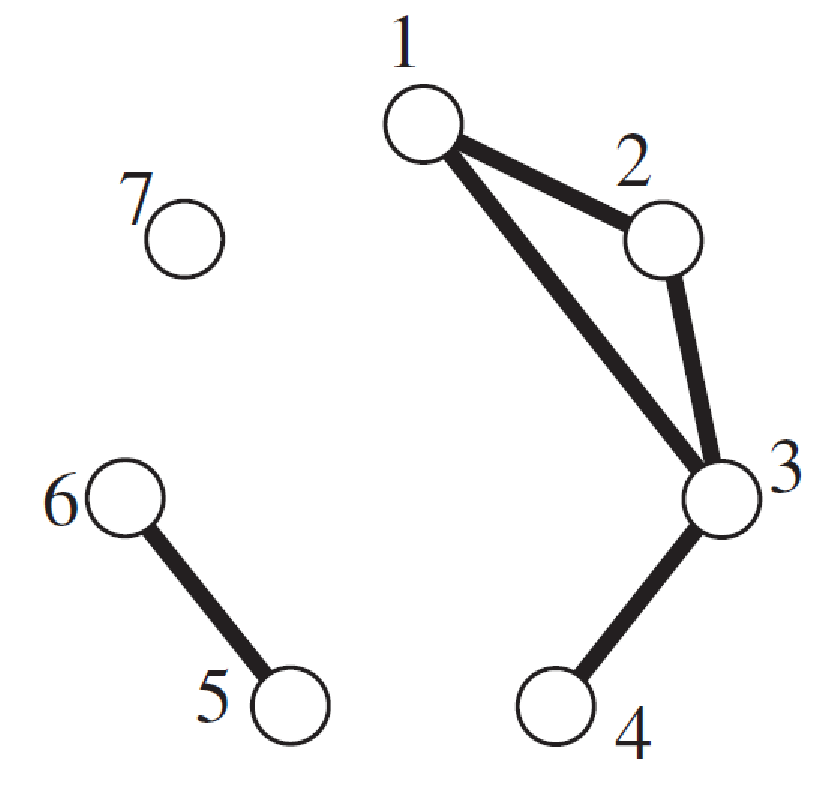
\includegraphics[scale=0.25]{Connected.pdf}
\end{figure}
\column{0.6\textwidth}
The equivalence classes are
\[
\{1,2,3,4\}\qquad \{5,6\}\qquad \{7\}
\]
Consider the induced subgraphs
\[
G[\{1,2,3,4\}]\qquad G[\{5,6\}]\qquad G[\{7\}]
\]
\end{columns}
\bl[Definition]{A \textbf{component} of $G$ is a subgraph of $G$ induced on an equivalence class of the is-connected-to relation on $V(G)$.}
\end{frame}

\begin{frame}
\bl[Definition]{A \textbf{component} of $G$ is a subgraph of $G$ induced on an equivalence class of the is-connected-to relation on $V(G)$.}
Extreme cases:
\itemb
\item In an edgeless graph, each of it's vertices forms a component unto itself.
\item It is possible that there is only one component.
\iteme

\bl[Definition]{A graph is called connected provided each pair of vertices in the graph is connected by a path; that is, for all $x,y\in V(G)$, there is an $(x,y)$-path.}
\begin{center}
Do Problem 2!
\end{center}
\end{frame}

\begin{frame}{Cut edges and cut vertices}
\bl[Definition]{Let $G$ be a graph. A vertex $v\in V(G)$ is a \textbf{cut vertex} of $G$ provided $G-v$ has more components than $G$. Similarly, an edge $e\in E(G)$ is called a \textbf{cut edge} of $G$ provided $G-e$ has more components than $G$.}
In the special case when $G$ is connected:
\itemb
\item A cut vertex $v$ is such that $G-v$ is disconnected.
\item An edge $e$ is a cut edge if $G-e$ is disconnected.
\iteme
However the cutting does not result in big disconnectedness.
\bl[Theorem]{Let $G$ be a connected graph and suppose $e\in E(G)$ is a cut edge of $G$. Then $G-e$ has exactly two components.} 
\end{frame}

\begin{frame}
\bl[Theorem]{Let $G$ be a connected graph and suppose $e\in E(G)$ is a cut edge of $G$. Then $G-e$ has exactly two components.} 
~~~~By the definition of a cutting edge, $G-e$ has at least two components. We will show that it has exactly two. 

~~~~FTSC assume that it is not so and let $a,b,c$ be three vertices of $G-e$, all in different components. This means that there is no path connecting any two of them.

~~~~Let $P$ be an $(a,b)$-path in $G$. Since this does not survive for $G-e$, $P$ must traverse $e$. Suppose that $e=xy$ and
\[
P=a\sim\dots\sim x\sim y\sim\dots\sim b.
\]
Similarly, since $G$ is connected, there is a $(c,a)$-path $Q$ from $c$ to $a$ that must use the edge $e=xy$. 

\center\textbf{Q}: Which vertex, $x$ or $y$ appears first \\ on $Q$ on the way from $c$ to $a$?
\end{frame}

\begin{frame}
\bl[Theorem]{Let $G$ be a connected graph and suppose $e\in E(G)$ is a cut edge of $G$. Then $G-e$ has exactly two components.} 
\textbf{Q}: Which vertex, $x$ or $y$ appears first \\ on $Q$ on the way from $c$ to $a$?

\itemb
\item If $x$ appears first, then the $(c,x)$ portion of $Q$ concatenated to the $(x,a)$-portion of $P^{-1}$ produces a $(c,a)$ walk in $G-e$. Therefore we also have a $(c,a)$ path in $G-e$, which contradicts the assumption. $\Rightarrow\Leftarrow$.
\iteme
\begin{figure}
\centering
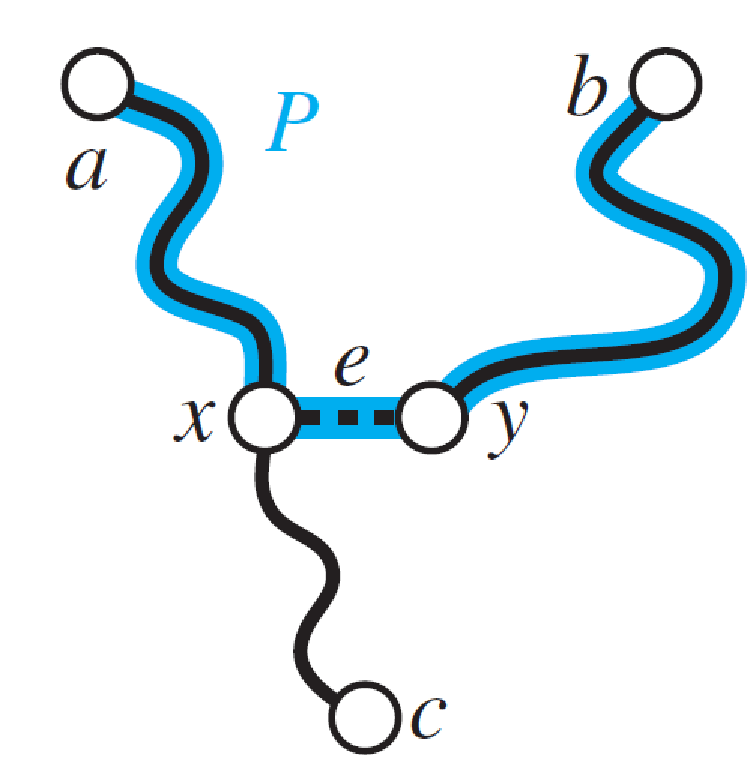
\includegraphics[scale=0.25]{Xfirst.pdf}
\end{figure}
\end{frame}

\begin{frame}
\bl[Theorem]{Let $G$ be a connected graph and suppose $e\in E(G)$ is a cut edge of $G$. Then $G-e$ has exactly two components.} 
\textbf{Q}: Which vertex, $x$ or $y$ appears first \\ on $Q$ on the way from $c$ to $a$?

\itemb
\item If $y$ appears first, then the $(c,y)$ portion of $Q$ concatenated to the $(x,b)$-portion of $P$ produces a $(c,b)$ walk in $G-e$. Therefore we also have a $(c,b)$ path in $G-e$, which contradicts the assumption. $\Rightarrow\Leftarrow$.
\iteme
\begin{figure}
\centering
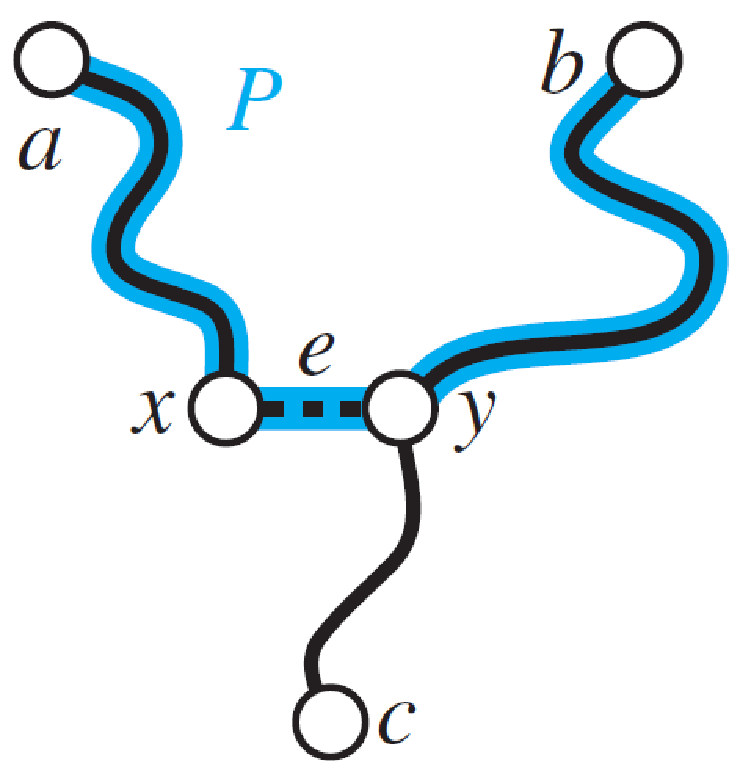
\includegraphics[scale=0.25]{Yfirst.pdf}
\end{figure}
\end{frame}

\begin{frame}
\begin{center}
Do Problem 3!
\end{center}
\end{frame}

\section{Trees}

\begin{frame}{Cycles}
\bl[Definition]{~~~~A \textbf{cycle} is a walk of length at least three in which the first and last vertex are the same, but no other vertices are repeated. \\
~~~~ The term can also refer to the (sub)graph consisting of the vertices and edges of such a walk. In other words, a cycle is a graph of the form $G=(V,E)$ where 
\[
V=\{v_1,v_2,\dots,v_n\},\qquad E=\{v_1v_2,v_2v_3,\dots,v_{n-1}v_n,v_nv_1\}.
\]}
\begin{figure}
\centering
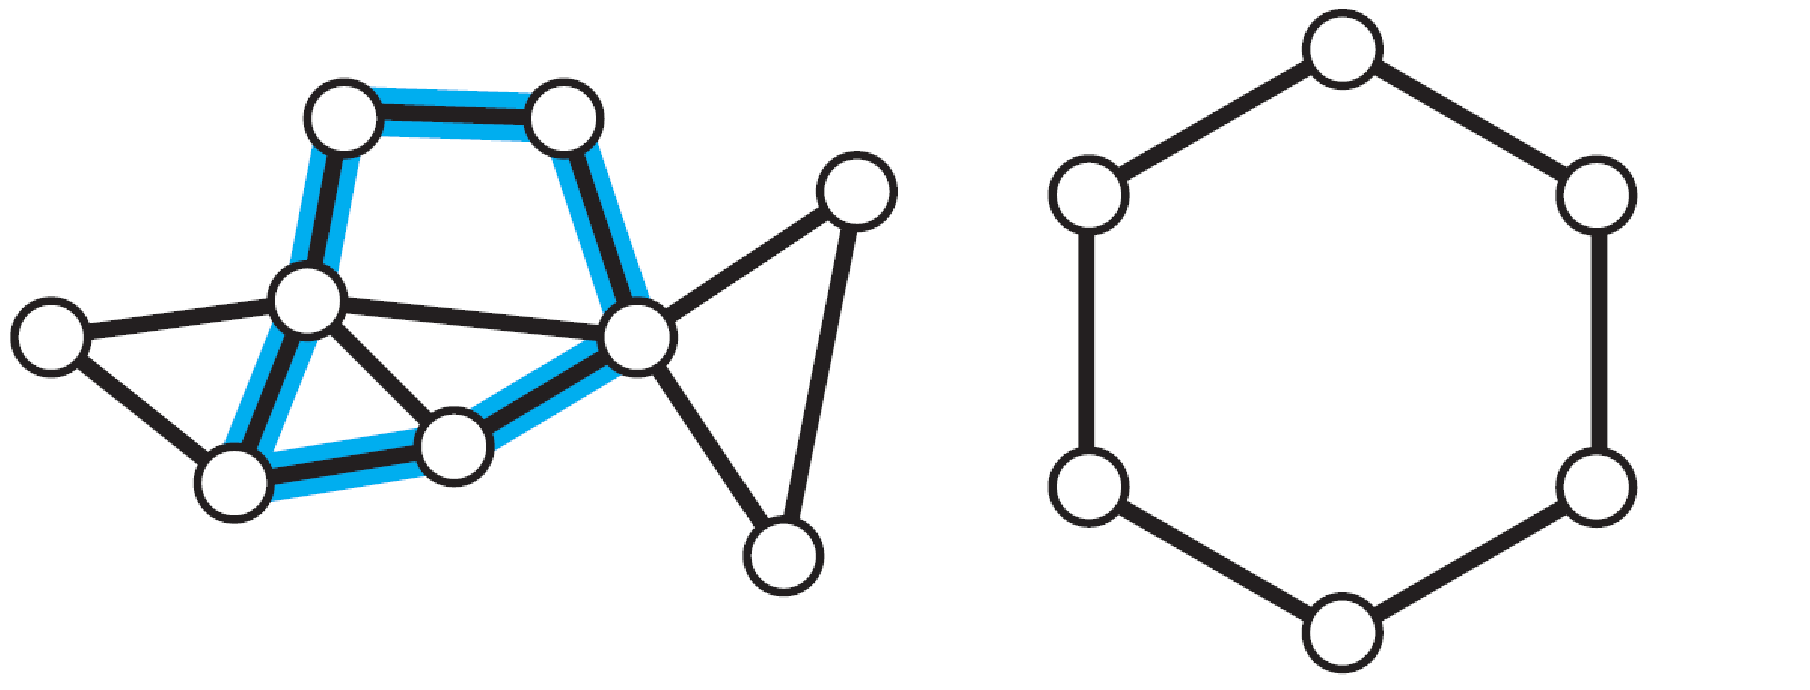
\includegraphics[scale=0.25]{Cycle.pdf}
\end{figure}\vspace{-0.5cm}
A cycle on $n$ vertices is denoted $C_n$.
\end{frame}

\begin{frame}{Forests and trees}
\bl[Definition]{Let $G$ be a graph. If $G$ contains no cycles, then we call $G$ \textbf{acyclic} or alternatively a \textbf{forest}.}
\bl[Definition]{A \textbf{tree} is a connected, acyclic graph.}
\begin{columns}
\column{0.4\textwidth}\vspace{-0.4cm}
\begin{figure}
\centering
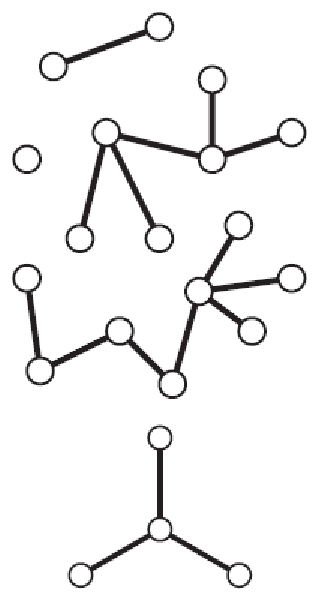
\includegraphics[scale=0.42]{Forest.pdf}
\end{figure}
\column{0.6\textwidth}
\itemb
\item A tree is a connected forest.
\item On the left is a forest with five components, all are trees.
\item Only tree on two vertices is $K_2$.
\item Trees on three and four vertices:
\iteme
\begin{center}
Do Problem 4!
\end{center}
\end{columns}

\end{frame}

\begin{frame}
\bl[Theorem]{Let $T$ be a tree. For any two vertices $a$ and $b$ in $V(T)$, there is a unique $(a,b)$ path. Conversely, any graph $G$ with this property must be  a tree.}
($\Rightarrow$) Suppose $T$ is a tree and let $a,b\in V(T)$. We need to prove that there is a unique $(a,b)$-path in $T$.

~~~~ Since $T$ is connected, there is at least one $(a,b)$ path. FTSC assume that there were two (or more) different $(a,b)$-paths $P$ or $Q$ in $T$; Let $x$ be the first place where they differ, i.e.
\[
P: a\sim\dots\sim x\sim\textcolor{blue}{y}\sim\dots\sim b,\qquad Q: a\sim \dots\sim x\sim\textcolor{blue}{z}\sim\dots\sim b
\]
This also means that the edge $xy$ cannot be in $Q$. Consider the graph $T-xy$.
\end{frame}

\begin{frame}
\bl[Theorem]{Let $T$ be a tree. For any two vertices $a$ and $b$ in $V(T)$, there is a unique $(a,b)$ path. Conversely, any graph with this property must be  a tree.}
Consider the graph $T-xy$.
\itemb
\item Consider the following $(x,y)$-walk in $T$. Start at $x$, follow $P^{-1}$ from $x$ to $a$, then follow $Q$ from $a$ to $b$ and then follow $P^{-1}$ from $b$ to $y$. This does not traverse $xy$ and therefore there is a walk and thus a path from $x$ to $y$ in $T-xy$ Call it $R$.
\item If we now concatenate $R$ and $xy$, we get a cycle in a tree which is impossible. $\Rightarrow\Leftarrow$
\iteme
($\Leftarrow$) FTSC assume that $G$ has a cycle. Then take two points $x$, $y$ on the cycle. Then clearly we have at least two ways to go from $x$ to $y$. (Two direction along the cycle.)$\Rightarrow\Leftarrow$.\qed

\end{frame}

\begin{frame}{Leafs}
\bl[Definition]{A \textbf{leaf} of a graph is a vertex of degree one.}
\bl[Theorem]{Every tree with at least two vertices has at least two leafs.}
Let $T$ be a tree with at least two vertices and let $P$ be a longest path in $T$. Then $P$ has two or more vertices, say
\[
P=v_0\sim v_1\sim\dots\sim v_l,\qquad l\geq 1.
\]
We claim that $v_0$ and $v_l$ must be leaves. If this was not so, then $v_0$ would have another neighbor $x$ that cannot be on $P$ because that would give a cylce. But then appending $x$ to the beginning of $P$ would give a longer path contradicting the maximality of $P$. Similar argument proves that $v_l$ is a leaf.
\end{frame}

\begin{frame}{Leafs}
\bl[Proposition]{Let $T$ be a tree and let $v$ be a leaf of $T$. Then $T-v$ is a tree.}
~~~~Clearly, $T-v$ cannot contain a cylce, because then the same cycle would be there in $T$ as well, which is impossible as $T$ is a tree.

~~~~To show that $T-v$ is connected, let $a,b\in V(T-v)$. Since $T$ is connected, there is an $(a,b)$ path $P$ in $T$. FTSC assume that
\[
P=a\sim\dots\sim v\sim\dots\sim b
\]
Since $v$ is not any of the endpoints, this would mean that $d(v)=2$, which is not the case as $v$ is a leaf. $\Rightarrow\Leftarrow$.  This means that $v$ cannot be on the path $P$ and therefore $P$ is an $(a,b)$-path in $T-v$ as well.

~~~~Since the choice of $a,b$ were arbitrary, $T-v$ is connected. This finishes the proof.\qed
\end{frame}

\begin{frame}{Further characterization of trees}
\bl[Theorem]{Let $G$ be a connected graph. Then $G$ is a tree if and only if every edge is a cutting edge.}
In this sense, trees are minimally connected graphs. For the proof, see the textbook.
\bl[Theorem]{Let $G$ be a connected graph on $n\geq 1$ vertices. Then $G$ is a tree if and only if $G$ has exactly $n-1$ edges.}

\begin{center}
Do Problem 5(a)
\end{center}
\end{frame}

\begin{frame}[t]{Spanning subgraphs}
\bl[Definition]{Let $G$ be a graph. A \textbf{spanning tree} of $G$ is a spanning subgraph of $G$ that is a tree.}
\bl[Theorem]{A graph has a spanning tree if and only if it is connected.}
\only<1>{($\Rightarrow$) Suppose $G$ has a spanning tree $T$. Let $u,v\in V(G)$. Since $T$ is spanning, we have $V(T)=V(G)$, and so $u,v\in V(T)$. Since $T$ is connected, there is a $(u,v)$-path $P$ in $T$. Since $T$ is a subgraph, $P$ is also a $(u,v)$-path of $G$.}

\only<2>{($\Leftarrow$) Suppose $G$ is connected. Let $T$ be a spanning connected subgraph of $G$ with the least number of edges. We claim that $T$ is a tree.

~~~~By construction, $T$ is connected. We show that every edge of $T$ is a cut edge. Otherwise, if $E(T)$ were not a cut edge of $T$, then $T-e$ would be a smaller spanning connected subgraph of $G$. $\Rightarrow\Leftarrow$.\qed}
\end{frame}
\begin{frame}
\begin{center}
Do Problem 5(b) and Problem 6
\end{center}
\end{frame}
\end{document}